\documentclass[tikz, border=5mm]{standalone}

\begin{document}
 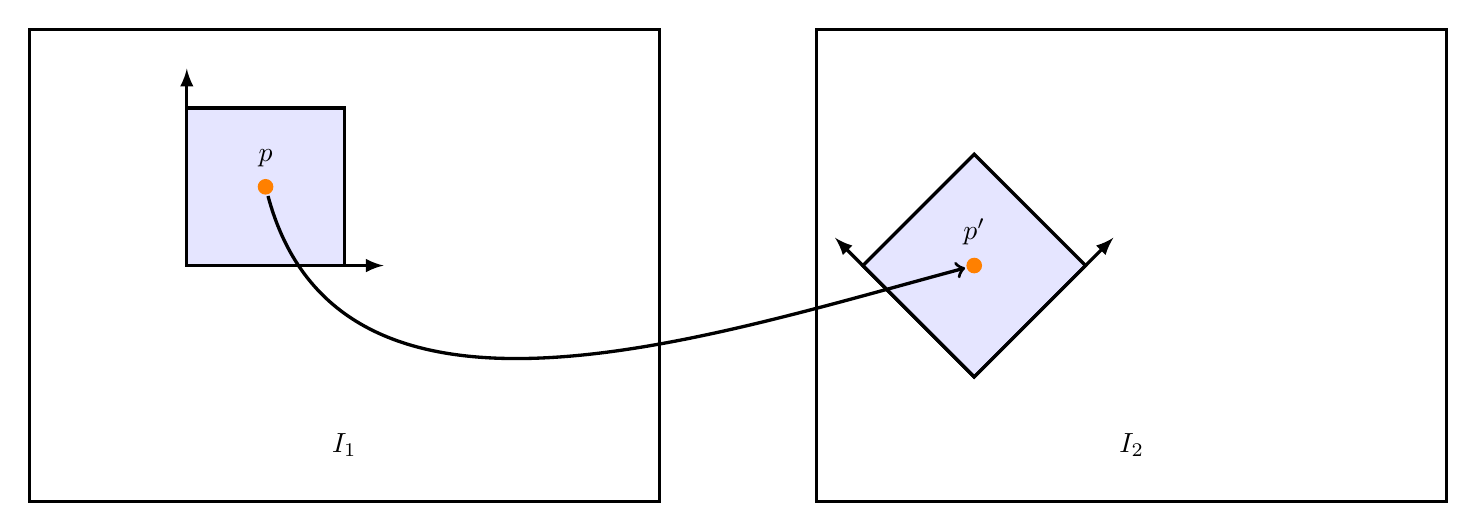
\begin{tikzpicture}[very thick]
 % plot two rectangles 8x6 separated in x 10 units
 \foreach \xoffset\lbl in {0/1,10/2} {
  \draw (\xoffset,0) rectangle ++(8,6) node [midway,below=2cm] {$I_\lbl$};
 }

 % define a new command named \Square with 4 arguments
 \newcommand{\Square}[4]{
  % Draw a square with {(x,y)}{rotation}{label}{name}
  \begin{scope}[shift={#1}, rotate=#2, >=latex]
   \draw [fill=blue!10!white] (-1,-1) rectangle (1,1) node [midway, circle, fill=orange, inner sep=2pt, label={90:{#3}}] (#4) {};
   \draw [<->] (1.5,-1) -- ++(-2.5,0) -- ++(0,2.5);
  \end{scope}
  }

  % Draw the squares and connect their centers
  \Square{(3,4)}{0}{$p$}{p1}
  \Square{(12,3)}{45}{$p'$}{p2}
  \draw [->] (p1) to [out=-75, in=195] (p2);
 \end{tikzpicture}
\end{document}